%% main_ppgco_ufu.tex v1.0, Lásaro Camargos e Denise Guliato
% adaptado de modeloABNT2.tex, v1.0 athila
% ------------------------------------------------------------------------
% ------------------------------------------------------------------------
% eesc: Modelo de Trabalho Acadêmico (tese de doutorado, dissertação de
% mestrado e trabalhos monográficos em geral) em conformidade com 
% ABNT NBR 14724:2011. Esta classe estende as funcionalidades da classe
% abnTeX2 elaborada de forma a adequar os parâmetros exigidos pelas 
% normas USP e do departamento de elétrica da Escola de Engenharia 
% de São Carlos - USP.
% ------------------------------------------------------------------------
% ------------------------------------------------------------------------
% Atualizações.
% 07/05/2015 - adicionada a seção de atualizações neste template.
% 18/11/2015 - atualizações para dissertações e teses com corpo em inglês
% 19/01/2021 - alterações nas referências com >3 autores (agora mostra todos)/
%              impressão de um lado somente
%              lista de algoritmos e lista de códigos
% ------------------------------------------------------------------------
% Opções:
% tesedr:     Formata documento para tese de doutorado
% qualidr:    Formata documento para qualificação de doutorado
% dissertmst: Formata documento para dissertação de mestrado
% qualimst:   Formata documento para qualificação de mestrado
% ------------------------------------------------------------------------
\documentclass[tesedr]{ppgco}
%Não altere o comando seguinte. O título de seu trabalho será especificado mais adiante.
\title{Template de Monografia do PPGCO}

% ---
% PACOTES
% ---

% ---
% Pacotes fundamentais 
% ---
%\usepackage{cmap}				% Mapear caracteres especiais no PDF
\usepackage{lmodern}				% Usa a fonte Latin Modern		
\usepackage{makeidx}            	% Cria o indice
\usepackage{hyperref}  			% Controla a formação do índice
\usepackage{lastpage}			% Usado pela Ficha catalográfica
\usepackage{indentfirst}			% Indenta o primeiro parágrafo de cada seção.
\usepackage{nomencl} 			% Lista de simbolos
\usepackage{graphicx}			% Inclusão de gráficos
\usepackage[portuguese]{babel}
\usepackage[brazil]{babel}
\usepackage{amsmath}
\newcommand*{\rttensor}[1]{\overline{\overline{#1}}}
\newcommand*{\rttensortwo}[1]{\bar{\bar{#1}}}
\newcommand{\VV}[1] {\vv{\vv{#1}}}
\newcommand{\mat}[1]{\mbox{\boldmath{$#1$}}}
\usepackage{physics}
% ---

% ---
% Pacotes adicionais, usados apenas no âmbito do Modelo eesc
% ---
\usepackage{lipsum}				       % para geração de dummy text
\usepackage[printonlyused]{acronym}

% ---


% ---
% Informações de dados para CAPA e FOLHA DE ROSTO
% ---
%
% Título:
%	1. Título em português
%	2. Título em inglês
\titulo{As quatro equações da fluidodinâmica e uma proposta para o tensor de tensões viscosas}

%
% Autor:
%	1. Nome completo do autor
%	2. Formato de nome para bibliografia
\autor{Ricardo Tadeu Oliveira Catta Preta \\matrícula: 11911FMT028}{Catta Preta, R.T.O}
%
% Cidade
\local{Uberlândia}
% Ano de defesa
\data{2022}
% Área de concentração da pesquisa
%\areaconcentracao{Física de Materiais}
% Nome do orientador
\orientador{Marcel Novaes}
% Nome do coorientador
%\coorientador{Nome completo do coorientador}
% ---

% ---
% compila o indice
% ---
\makeindex
% ---

% ---
% Compila a lista de abreviaturas e siglas
% ---
\makenomenclature
% ---

% ---
% Inserir ficha catalográfica
%
% Caso o comando \inserirfichacatalografica seja definido, a %ficha catalográfica
% será inserida atrás da folha de rosto. Caso contrário a página será deixada em
% branco.
%
% CUIDADO: Esta opção deve ser preenchida antes do comando \maketitle
% ---
%entre em contato com a biblioteca para obter a sua ficha catalográfica em arquivo pdf. Essa %folha só será inserida no documento após a sua defesa.

%\inserirfichacatalografica{fichaCatalografica.pdf}
% ---

% ----
% Início do documento
% ----

\begin{document}

% elementos pré-textuais ainda estão em inglês no template, voltando para ptbr
\renewcommand{\orientadorname}{Orientador: }
\renewcommand{\coorientadorname}{Coorientador: }
\renewcommand{\agradecimentosname}{Agradecimentos}

% ----------------------------------------------------------
% ELEMENTOS PRÉ-TEXTUAIS
% ----------------------------------------------------------
\pretextual

% ---
% Insere Capa, Folha de rosto, Ficha catalográfica (se inserida)
% e folha de aprovação (se inserida).
% ---
\maketitle


% ---
% Dedicatória
% ---
%\imprimirdedicatoria{Este trabalho é dedicado às crianças adultas %que,\\
%   quando pequenas, sonharam em se tornar cientistas.}
% ---

% ---
% Agradecimentos
% ---
\imprimiragradecimentos{
Agradeço a meu amigo Maurício, por ter me influenciado a tomar a melhor decisão da minha vida (fazer o curso de física). Agradeço aos meus amigos, Alejandro, Igor Baratta, Dani e o Vini, pela incrível paciência de me escutar falando sobre física. Sem a reflexão com estes amigos meu caminho seria completamente diferente. Agradeço à minha mãe, irmãs e família, por sempre me apoiar com a busca deste sonho. Obrigado ao professor Marcel Novaes, pela oportunidade  de me orientar com dicas decisivas para os conceitos abordados no TCC. Muito obrigado aos amigos do grupo do almoço (turma da física) pela ajuda e companheirismo ao longo do curso. Saúdo os amigos que compartilham a vida comigo, em especial, dos grupos: música satânica, clube do dreher, Tchoflotoni Conection, almoço satânico, climbUdão, Lunáticos, MFLab, Insanos, Cs anápolis e aglomerados, Azeitonas, Xadrez satânico e EPTT satânico. 
}
% ---

% ---
% Epígrafe
% ---
%\imprimirepigrafe{
%		``Sua vida pode ser dividida em dois períodos: antes de %agora e a partir de agora.''\\
%		(Prof. Obvious Stating)
%}
% ---

% ---
% RESUMO e ABSTRACT
% ---

% Resumo em português - as palavras entre chaves são as palavras-chave do trbalho
\begin{comment}

\begin{resumo}{Latex. Abntex. Normas USP}

 	 Segundo a \citeonline[3.1-3.2]{NBR6028:2003}, o resumo deve ressaltar o  objetivo, o método, os resultados e as conclusões do documento. A ordem e a extensão  destes itens dependem do tipo de resumo (informativo ou indicativo) e do  tratamento que cada item recebe no documento original. O resumo deve ser  precedido da referência do documento, com exceção do resumo inserido no  próprio documento. (\ldots) As palavras-chave devem figurar logo abaixo do  resumo, antecedidas da expressão Palavras-chave:, separadas entre si por  ponto e finalizadas também por ponto.
     
    Para auxiliá-lo com o latex, o Apêndice 
  \ref{cap_exemplos} apresenta os resultados dos comandos incluídos no arquivo ape\_comandos/abntex2-modelo-include-comandos.tex 

\end{resumo}
\end{comment}

%\selectlanguage{portuguese}
%\usepackage[T1]{fontenc} 
%\usepackage[utf8]{inputenc}

%% página com título em Inglês
\imprimiringlescapa

% Inserir folha de aprovação en Inglês
%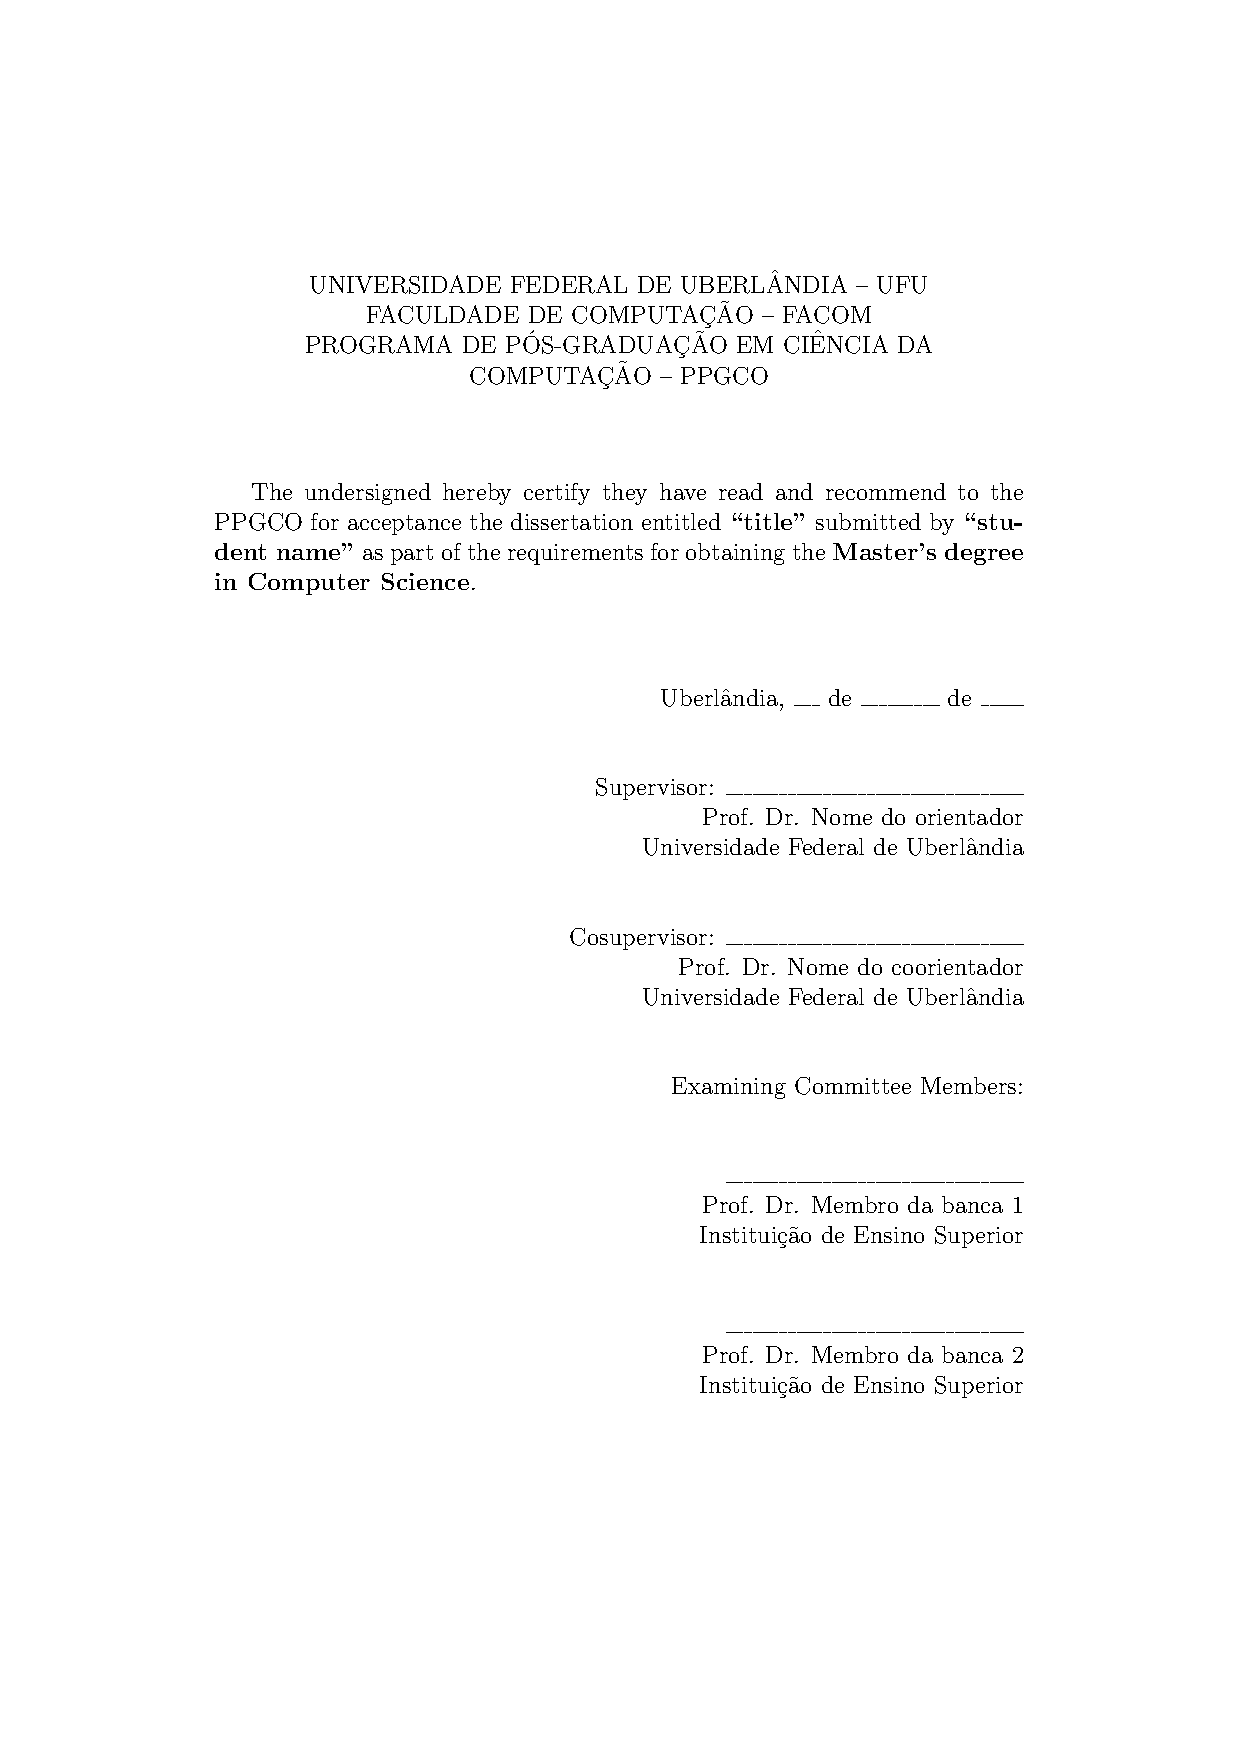
\includepdf[pages={1}]{folhaAprovacao.pdf}

% Resumo em inglês
\begin{comment}

\begin{abstract}{Latex. Abntex.}
This is the English abstract.
\end{abstract}
\end{comment}

% ---

% ---
% inserir lista de ilustrações
% ---
%\listailustracoes
% ---

% ---
% inserir lista de tabelas
% ---
%\listatabelas
% ---

% ---
% inserir lista de códigos (específicos de linguagens)
% ---
%\listadecodigos

% ---
% inserir lista de algortimos (pseudocódigos)
% ---
%\listadealgoritmos

% ---
% inserir lista de abreviaturas e siglas
% ---
%\listasiglas{abrev/Abreviaturas}
% ---

% ---
% inserir o sumario
% ---
\sumario
% ---

% ----------------------------------------------------------
% ELEMENTOS TEXTUAIS
% ----------------------------------------------------------
\mainmatter


% ----------------------------------------------------------
% Copyright
% ----------------------------------------------------------
\begin{comment}

\newpage
\thispagestyle{empty}

\ \

\vspace{10cm}

I hereby certify that I have obtained all legal permissions from the owner(s) of each third-party copyrighted matter included in my thesis, and that their permissions allow availability such as being deposited in public digital libraries.

\vspace{5cm}

\begin{center}
student name and signature
\end{center}

\end{comment}

% ----------------------------------------------------------
% Introdução
% ----------------------------------------------------------
\chapter[Introdução]{Introdução}

\section{Uma breve introdução à história das equações de Navier-Stokes }

Isaac Newton pode ser considerado como o pai da mecânica dos fluidos. Foi o primeiro a publicar artigos sobre a descrição do movimento dos fluidos através de equações diferenciais. O livro 2 do famoso \emph{Principia}, em que Newton descreve as propriedades dos fluidos e sua interação com os corpos imersos, consistiu em resultados originais para a época \cite{truesdell1953notes}. Newton abria mais um novo campo na física. Porém, os resultados experimentais não fechavam bem com sua teoria proposta. Coube à Academia de Berlim, em 1748, propor uma competição para premiar, em 1750, quem descrevesse a melhor teoria sobre os fluidos. Interessante reparar a ingenuidade dos organizadores em pensar que em apenas dois anos poderia haver uma teoria satisfatória para esse tema. Importante observar também como o apoio à pesquisa em universidades pode contribuir para avanços na área tecnológica.

Grandes nomes da história da física e da matemática contribuíram para o desenvolvimento das equações da dinâmica dos fluidos: I. Newton, D. Bernoulli, J. L. d'Alambert, Leonard Euler, C. L. M. H. Navier, A. Cauchy, S.D. Poisson e G. G. Stokes, por exemplo. As principais contribuições serão apresentadas a seguir.
\subsection{Convenção da notação utilizada}
O uso da notação indicial com o cálculo tensorial facilita a álgebra dos tensores apresentados ao longo do trabalho. Para um melhor entendimento do cálculo tensorial, existe uma vasta literatura \cite{aris2012vectors}, \cite{jeffreys1961cartesian}, \cite{arfken1999mathematical} e \cite{morse1953mathematical}. Neste estudo será utilizada a convenção de soma de Einstein sempre que for conveniente, com uma nomenclatura que pode ser revista em \cite{frisch1995turbulence}. Assim, os operadores diferencias assumem a forma:
\begin{equation}
\dd_{t} \equiv \frac{\dd}{\dd t}, \quad
    \partial_{t} \equiv \frac{\partial}{\partial t}, \quad \partial_{i} \equiv \frac{\partial}{\partial x_{i}}, \quad \partial_{ij} \equiv \frac{\partial^2}{\partial x_{i}\partial x_{j}}.  
\end{equation}

\subsection{I. Newton}
Em 1687, com seu livro \emph{Principia}, Newton foi o primeiro a considerar matematicamente o fluido como contínuo (sem espaços vazios). Newton percebeu a relação linear que existe entre as tensões de cisalhamento do fluido e o gradiente de velocidade. Futuramente a classe de fluidos que seguem essa característica ficou conhecida como fluidos newtonianos. Em outras palavras, Newton propôs um modelo linear para as tensões viscosas em função do gradiente de velocidade, e o fator de proporcionalidade ficou conhecido como viscosidade molecular. 

O modelo proposto por Newton parte de um campo de velocidade $\textbf{V}(x, y, z) = u \textbf{i} + v\textbf{j} + w\textbf{k}$, onde $\textbf{i}$, $\textbf{j}$ e $\textbf{k}$ são os vetores unitários ortogonais nas direções $x$, $y$ e $z$ respectivamente; $u$, $v$ e $w$ são os componentes do campo de velocidade e também são função de $x$, $y$ e $z$. A hipótese proposta parte de um escoamento bidimensional e ocorre apenas na direção $x$. A viscosidade de Newton é apresentada como
\begin{equation*}
    \tau = \mu\frac{du(y)}{dy},
\end{equation*}
onde $\tau$ é a tensão de cisalhamento, sendo a força por unidade de área; $\mu$ é a viscosidade molecular do fluido (considerada constante); $u(y)$ é função apenas de $y$.

Essa contribuição dada por Newton foi de extrema importância para o desenvolvimento da dinâmica dos fluidos. Futuramente essa hipótese foi alterada pelo matemático e físico escocês G. G. Stokes, que a generalizou.

\subsection{D. Bernoulli}
Em 1738, com seu livro intitulado \emph{Hydrodynamic}, D. Bernoulli publicou um importante teorema para os fluidos invíscidos (fluidos sem viscosidade),
\begin{equation}
    p + \frac{1}{2}\rho v^2 + \rho g= C,
\end{equation}
sendo $p$ a pressão mecânica exercida, $\rho$ a densidade, $\frac{1}{2}\rho v^2$, a energia cinética específica do fluido, $\rho g$ a energia potencial gravitacional específica, e $C$ uma constante. Essa equação teve um impacto muito forte, por ser muito simples mas ter inúmeras aplicações na engenharia. 

Entretanto, como essa equação só vale para fluidos sem viscosidade, ocorrem erros em muitas situações práticas ao aplicá-la, pois, como veremos mais a frente, não existe fluido com viscosidade zero (em um nível macroscópico).
\subsection{L. Euler}
Entre os anos de 1755 e 1757, foi a vez do grande matemático Leonard Euler dar uma contribuição revolucionária para a dinâmica dos fluidos. Euler propôs duas equações que podem ser utilizadas para escoamentos compressíveis e incompressíveis. Tais equações, apresentadas abaixo, ficaram conhecidas como equação da continuidade e equação de Euler, respectivamente:
\begin{align*}
    \partial_t \rho + \nabla \cdot (\rho\textbf{V}) &= 0,\\
    \partial_t \textbf{V} + (\textbf{V}\cdot\nabla)\textbf{V} &=-\frac{1}{\rho} \nabla p + \textbf{g},
\end{align*}
onde $p$ é o campo de pressão exercido sobre a partícula de fluido, e $\textbf{g}$ é a aceleração da gravidade. 

A equação da continuidade é bem entendida. Já a equação de Euler, também conhecida como a equação de transporte de momentum, tem do lado esquerdo da igualdade a soma de duas formas de aceleração. A primeira é uma aceleração que ocorre em um ponto fixo do espaço e a segunda que pode variar ao longo do espaço, mesmo que o tempo esteja fixo. O lado direito da equação de Euler tem um termo que é menos o gradiente de pressão, ou seja, diz que o escoamento se move sempre da maior para menor pressão, e o termo da aceleração da gravidade. O avanço na representação da dinâmica dos fluidos embutida nessa equação de transporte de momentum se deve principalmente ao fato do aparecimento do termo não linear (ou seja, aparece um termo proporcional a $v^2$). A não linearidade é uma das características mais marcantes nos escoamentos turbulentos — sendo o comportamento dos fluidos em sua forma caótica. 

Até a presente data da publicação deste estudo, ninguém conseguiu provar a existência e unicidade das soluções gerais desse sistema de equação (dadas as devidas condições de contorno e iniciais) \cite{fefferman2000existence}.

As equações de Euler são utilizadas para os fluidos ditos ideais — fluidos com viscosidade zero. Um importante resultado é que a integração dessas equações sobre um dado volume recai na equação proposta por D. Bernoulli. 

É interessante ressaltar que a versão mais detalhada das equações da dinâmica dos fluidos (equações de Navier-Stokes), mesmo envolvendo um termo a mais, o termo viscoso, ainda é menos complexa do que as equações de Euler \cite{stewart2013great}. Uma das principais dificuldades de se obter as soluções das equações de Euler está no fato das soluções facilmente explodirem para infinito, justamente pela falta de um termo de amortecimento \cite{stewart2013great}. 

\subsection{C.-L.-M.-H. Navier}
Foi em 1822 que o físico e engenheiro naval Navier propôs o termo que faltava para descrever o escoamento dos fluidos viscosos. A contribuição de Navier foi apenas para fluidos newtonianos e incompressíveis, mas mesmo assim foi um enorme avanço para a dinâmica dos fluidos. O termo viscoso proposto é proporcional ao laplaciano da velocidade, como apresentado abaixo
\begin{align*}
    \nabla \cdot \textbf{V} &= 0,\\
    \partial_t \textbf{V} + (\textbf{V}\cdot\nabla)\textbf{V} &=-\frac{1}{\rho} \nabla p + \nu \nabla^2\textbf{V} + \textbf{f},
\end{align*}
onde $\nu$ é a viscosidade cinemática do fluido e $\textbf{f}$ uma força de campo que estiver atuando sobra a partícula de fluido.

A introdução do termo viscoso introduz sérias modificações no comportamento da equação de transporte de momentum. Listaremos algumas das principais. Primeiramente, a equação diferencial parcial agora é de segunda ordem. Assim, necessita-se de uma condição de contorno a mais, quando comparada com a equação de transporte de momentum proposta por Euler. Outra importante mudança reside no fato da perda da simetria temporal da equação. A equação de Euler é invariante sob uma inversão temporal, ou seja, a transformação $t\longrightarrow -t$ para as coordenadas que dependem do tempo, não altera a equação \cite{frisch1995turbulence}. O mesmo não é possível com as novas equações de Navier. A introdução do termo viscoso quebra a simetria temporal.

Sabemos pelos teoremas de Emmy Noether \cite{lemos2007mecanica, goldstein2002classical} que uma simetria temporal está relacionada com a conservação de energia. Assim, chegamos à conclusão que adicionar o termo viscoso, por conseguinte, perder a importante característica de simetria temporal, era o que faltava para conseguirmos resultados mais coerentes entre a previsão teórica e os resultados experimentais.

Particularmente, entendo que esse é o preço que pagamos por tentar modelar um efeito que é molecular, através de variáveis macroscópicas. Precisamos ressaltar que as variáveis do campo de velocidade e campo de pressão são variáveis médias — como demonstraremos com a equação de transporte de Boltzman. Nessa transferência de informação de quantidades moleculares para a escala macro ocorrem perdas, o que é totalmente condizente com a segunda lei da termodinâmica.

\subsection{A. Cauchy}
Quando Cauchy contribuiu para a dinâmica dos fluidos (1828), seu interesse inicial estava em aplicações da teoria óptica. Ele fez grandes esforços para criar uma teoria elástica da luz. Portanto, foi com analogias no campo da óptica que acabou surgindo uma proposta original sobre o comportamento das tensões sobre um fluido.

A principal diferença da proposta de Cauchy para as equações de transporte de momentum de Euler e Navier está no conceito de pressão interna. A nova proposta seria que o tensor de tensões viscosas fosse proporcional a um gradiente de velocidade, sendo o fator de proporcionalidade um tensor isotrópico de quarta ordem. A apresentação do tensor será feita em seções seguintes. Agora iremos apresentar apenas a versão final do tensor
\begin{equation*}\label{NS_final}
\partial_{t}(\rho u_{i})+ \partial_{j} (\rho u_{j}u_{i})=  \partial_{j}\sigma_{ij},
\end{equation*}
onde $\sigma_{ij} = \left[\mu\left(\partial_{j}u_{i} + \partial_{i}u_{j}\right) + \lambda\partial_{k}u_{k}\delta_{ij}\right]$, $\mu$ é a viscosidade dinâmica do fluido e $\lambda$ é conhecido como o segundo coeficiente de viscosidade.

Quando é aplicado o operador divergente sobre o termo $\lambda\partial_{k}u_{k}\delta_{ij}$, obtemos o gradiente de $\lambda\partial_{k}u_{k}$, que tem uma natureza bem próxima da pressão. Cauchy chamou esse tensor de pressão interna, e entendeu que a pressão mecânica que vinha nas equações de Euler e Navier eram desnecessárias e isso ajudaria a diminuir uma incógnita do problema. Porém, sua interpretação foi falha nesse aspecto, como constataremos na proposta de Poisson.
\subsection{S. D. Poisson}

Em 1829, Poisson percebeu o avanço proposto por Cauchy e identificou o erro cometido ao descartar a importância da pressão mecânica. Assim, a equação proposta por Poisson é a equação de Cauchy acrescentada do termo do gradiente de pressão
\begin{equation*}\label{Poisson}
\partial_{t}(\rho u_{i})+ \partial_{j} (\rho u_{j}u_{i})= -\partial_{i}p + \partial_{j}\left[\mu\left(\partial_{j}u_{i} + \partial_{i}u_{j}\right) +\lambda\partial_{k}u_{k}\delta_{ij}\right].
\end{equation*}

\subsection{G. G. Stokes}
Finalmente chegamos na última grande contribuição para a dinâmica dos fluidos newtonianos. Em 1845, o físico e matemático G. G. Stokes propôs \cite{stokes2007theories} uma hipótese para eliminar o segundo coeficiente de viscosidade proposto por Cauchy e, assim, ter uma descrição completa do ponto de vista macroscópico dos fluidos newtonianos compressíveis e incompressíveis. A hipótese acabou ficando conhecida como "a hipótese de Stokes" e consiste em estabelecer uma relação entre a viscosidade dinâmica e o segundo coeficiente de viscosidade. Após algumas considerações matemáticas, Stokes estabeleceu que $\lambda = - \frac{2}{3}\mu$. A dedução detalhada desta hipótese será apresentada na seção seguinte.

Para mais detalhes sobre a contribuição de cada um desses grandes cientistas, recomento a leitura de \cite{truesdell1953notes}. Neste trabalho, será enfatizada apenas a versão mais atual e completa dessas equações, proposta em definitivo por Stokes.

\section{Dedução das equações da mecânica dos fluidos} 
As equações da mecânica dos fluidos são um conjunto de equações da mecânica dos meios contínuos. Para identificarmos se o escoamento está na hipótese do contínuo, temos o número adimensional de  Knudsen $Kn = \frac{\lambda}{L}$, onde $\lambda$ é o livre caminho médio molecular e $L$ é a escala de comprimento físico que está sendo representada. Se a hipótese do contínuo é válida, é preciso que do ponto de vista numérico $Kn < 0,01$ \cite{karniadakis2006microflows}. 

Para apresentarmos as equações da dinâmica dos fluidos, iremos discutir como as variáveis de campo contínuo são valores médios. Quando observamos do ponto de vista macroscópico um fluido escoando em regime laminar, os valores dos campos de velocidade, pressão, e densidade são valores médios, na verdade. As moléculas que constituem o fluido possui um movimento aleatório quando observadas na meso-escala. Porém, quando observadas na macroescala, a aleatoriedade é perdida. A passagem da meso-escala para a macro escala requer uma descrição estatística do fluido. Para isso, temos a função de distribuição $f(t, x_i, p_i)$ das moléculas de um fluido no seu espaço de fase. Em geral, a função depende do tempo, das coordenadas da posição ($x_i$) e do momento ($p_i$). Seja $d\tau = dx_{i}dp_i$ o elemento de volume no espaço de fase do fluido. O produto $fd\tau$ é o número médio de moléculas em um dado elemento $d\tau$ que tem valores $x_i$ e $p_i$ nos intervalos $dx_i$ e $dp_i$. 

Chamaremos por $\Gamma$ o conjunto de todas as variáveis em que a função de distribuição depende. Nós separamos do elemento de volume de fase $\dtau$ o fator $dV = dxdydz$, e denotamos por $d\Gamma$ o restante das variáveis usadas. As quantidades $\Gamma$ tem três componentes do momentum $\textbf{p} = m\textbf{v}$ da partícula de fluido, assim $d\Gamma = d^{3}p$ \cite{pitaevskii2012physical}.

A densidade de distribuição espacial das moléculas que constituem o fluido é
\begin{equation}
    N(t, x_{i}) = \int_{\Gamma} f(t, x_{i}, \Gamma) \dd\Gamma,
\end{equation}
sendo que o produto $NdV$ é o número médio de partículas de fluido em um dado volume $dV$.

A dedução que faremos para as equações será uma extensão da dedução apresentado por \cite{pitaevskii2012physical}. Digo uma extensão pelo fato do Landau não deduzir a parte do tensor de tensões viscosas. O procedimento será por meio da equação de transporte de Boltzman \cite{landau2013course}
\begin{equation}\label{boltzman_eq}
    \partial_{t} f + \partial_{j}(v_{j}f) = C(f),
\end{equation}
onde $f$ é a função densidade de probabilidade, $C(f)$ é a taxa de mudança da função densidade de probabilidade devida às colisões que ocorrem na escala abaixo do contínuo. Por fim, $v_{j}$ são as componentes da velocidade das partículas transportadas.

 As propriedades macroscópicas do fluido, digamos $\Bar{\phi}(t, x_{i})$, podem ser calculadas de forma geral, como:
\begin{equation}
    \Bar{\phi}(t, x_{i}) = \frac{1}{N(t, x_{i})} \int_{\Gamma} \phi(t, x_{i}, \Gamma) f(t, x_{i}, \Gamma) \dd\Gamma.
\end{equation}

Por exemplo, a partir da velocidade microscópica do fluido ($v_{i}$), podemos calcular a velocidade macroscópica $(u_{i})$,
\begin{equation}\label{velocity_filter}
    u_{i} = \Bar{v}_{i} = \frac{1}{N} \int_{\Gamma} v_{i}f \dd\Gamma.
\end{equation}

Assumiremos que as colisões entre as moléculas não alteram o número de partículas que estão colidindo nem a quantidade total de energia e momentum do sistema \cite{pitaevskii2012physical}. Em resumo, não consideraremos que $C(f)$ possa alterar as quantidades macroscópicas de cada elemento de volume do fluido, i.e. — densidade, energia interna, e velocidade macroscópica.
\begin{equation}
\int_{\Gamma} C(f) \dd\Gamma = 0,
\end{equation}
\begin{equation}
\int_{\Gamma} e C(f) \dd\Gamma = 0,
\end{equation}
\begin{equation}\label{momentum_conservation}
\int_{\Gamma} P_{i}C(f) \dd\Gamma = 0,
\end{equation}
onde $e$ e $P_{i} = mv_{i}$, são respectivamente, a energia interna e a quantidade de movimento das moléculas do fluido.
\section{Equação da continuidade}
Podemos deduzir a equação da continuidade por meio da equação \ref{boltzman_eq}. Para isso, precisamos multiplicar toda a equação pela massa da partícula de fluido $m$, e posteriormente, integrar toda a equação em $\dd\Gamma$.
\begin{equation}
\int_{\Gamma}[m\partial_{t}f + m\partial_{j}(v_{j}f) ]\dd\Gamma = m\int_{\Gamma} C(f) \dd\Gamma.
\end{equation}

Utilizando as propriedades apresentadas na seção anterior, e assumindo que a função de distribuição e a massa da partícula são contínuas.
\begin{equation*}
\partial_{t}\int_{\Gamma}mf\dd\Gamma + \partial_{j} \int_{\Gamma}(mv_{j}f)\dd\Gamma = 0
\end{equation*}
\begin{equation*}
\partial_{t}(mN)+ \partial_{j} (mNu_{j})= 0,
\end{equation*}
sendo $\rho = mN$, a massa específica do volume de fluido. Ou seja
\begin{equation}\label{continuity_eq}
\partial_{t}\rho+ \partial_{j} (\rho u_{j})= 0.
\end{equation}

A equação da continuidade pode ser bem interpretada na sua forma integral. Ao integrarmos a equação \ref{continuity_eq} ao longo do volume macroscópico “infinitesimal”, $\dd V$, e utilizando o teorema de Gauss-Ostrogradsky: 
\begin{equation*}
\partial_{t}\int_{V}\rho \dd V = -\oint_{\partial V} \rho u_{j} \,ds_{j},
\end{equation*}
podemos interpretar que a taxa de variação da massa em um determinado volume, muda com o fluxo dos componentes da densidade de quantidade de movimento que atravessa a superfície que delimita o volume $\dd V$.

\section{Equações de Navier-Stokes}
O ponto de partida para a dedução das equações de Navier-Stokes (N-S) também se dá pela equação de transporte de Boltzman. Sabendo da conservação da quantidade de movimento das partículas que constituem o fluido, multiplicamos toda a equação \ref{boltzman_eq} por $mv_{i}$, e posteriormente integramos 
\begin{equation*}
\int_{\Gamma}[mv_{i}\partial_{t}f + mv_{i}\partial_{j}(v_{j}f) ]\dd\Gamma = \int_{\Gamma} mv_{i}C(f) \dd\Gamma
\end{equation*}
\begin{equation*}
\int_{\Gamma}[\partial_{t}(mv_{i}f) + \partial_{j}(mv_{i}v_{j}f) ]\dd\Gamma = \int_{\Gamma} mv_{i}C(f) \dd\Gamma,
\end{equation*}
e usando as propriedades \ref{momentum_conservation} e \ref{velocity_filter}, temos
\begin{equation*}
\partial_{t}(mNu_{i})+ \partial_{j} (mN\overline{v_{j}v_{i}})= 0,
\end{equation*}
ou
\begin{equation}\label{NS_f1}
\partial_{t}(\rho u_{i})+ \partial_{j} (\rho\Pi_{ij})= 0,
\end{equation}
onde $\rho = mN$ e $\Pi_{ij} = \overline{v_{j}v_{i}}$, são os componentes do tensor fluxo de quantidade de movimento \cite{pitaevskii2012physical}.

Agora chegamos no momento de decompor o tensor \boldsymbol{\Pi}. É interessante observar que o procedimento de filtragem das propriedades da meso-escala quando transportadas para a escala macroscópica é idêntico à Simulação das Grandes Escalas, termo em inglês para Large Eddy Simulation (LES) — método de modelagem do fenômeno da turbulência \cite{catta2018implementaccao}, \cite{sagaut2006large} e \cite{pope2000turbulent}.

Para realizar a decomposição do tensor \boldsymbol{\Pi}, precisamos decompor o campo de velocidade das partículas que constituem o fluido. A decomposição é feita com uma parcela média $u_{i}$ e uma parcela flutuante $v^{'}_{i}$. De forma que $v_{i} = u_{i} + v^{'}_{i}$.
\begin{equation}
\begin{split}
\Pi_{ij} = & \overline{v_{j}v_{i}} \\
= &\overline{(u_{i} + v^{'}_{i})(u_{j} + v^{'}_{j})} \\
=& u_{i}u_{j} + \overline{v^{'}_{i}v^{'}_{j}}.
\end{split}
\end{equation}

As propriedades de filtragem utilizadas acima podem ser conferidas em diversas referências, como \cite{catta2018implementaccao}, \cite{sagaut2006large}, \cite{pitaevskii2012physical} e \cite{pope2000turbulent}.

Agora podemos reescrever a equação \ref{NS_f1} como: 
\begin{equation}\label{NS_f2}
\partial_{t}(\rho u_{i})+ \partial_{j} (\rho u_{j}u_{i})= \partial_{j} \sigma_{ij},
\end{equation}
onde $\sigma_{ij} = -\overline{v^{'}_{i}v^{'}_{j}}$, são os componentes do tensor de tensões que atua na superfície da partícula de fluido na escala macroscópica. Tensor \boldsymbol{\sigma} precisa ser modelado, e sua forma definitiva foi proposta por \cite{stokes2007theories}. Porém, aqui será apresentada uma dedução mais moderna e completa, muito bem discutida em \cite{batchelor2000introduction}.

O tensor de segunda ordem $\boldsymbol{\sigma}$ pode ter suas componentes decompostas em uma parte isotrópica $(\frac{1}{3}\sigma_{kk}\delta_{ij})$ — sendo $\delta_{ij}$ os componentes do tensor delta de Kronecker — e outra parte chamada deviatórica $(\sigma^{d}_{ij})$, tal que \cite{batchelor2000introduction}, 
\begin{equation}\label{sigma_1}
\sigma_{ij} = \frac{1}{3}\sigma_{kk}\delta_{ij} + \sigma^{d}_{ij}.
\end{equation}

Analisaremos inicialmente a parte isotrópica. Temos que $\sigma_{kk} = -\overline{v^{'}_{k}v^{'}_{k}}$, e, $\frac{1}{3}\overline{v^{'}_{k}v^{'}_{k}}$ é a filtragem da média do quadrado das flutuações das velocidades das partículas que constituem o fluido. Do ponto de vista da mecânica estatística, isso pode ser modelado como a pressão que as partículas de fluido exercem sobre a superfície, onde $p = \frac{1}{3}\overline{v^{'}_{k}v^{'}_{k}}$. Assim, a parte isotrópica do tensor $\boldsymbol{\sigma}$ pode ser modelada como $-p\delta_{ij}$.

Agora podemos passar para a componente deviatórica do tensor $\boldsymbol{\sigma}$. Muitas vezes referido como tensor de tensões viscosas \cite{landau2013fluid}, \cite{white2006viscous}, $\boldsymbol{\sigma^{d}}$, é normalmente dado pelo símbolo $\boldsymbol{\tau}$. Tais tensões são resultantes da transferência irreversível do fluxo de quantidade de movimento devido aos choques moleculares que ocorrem quando temos velocidades relativas entre as moléculas que constituem o fluido \cite{landau2013fluid}. Em outras palavras, o tensor $\boldsymbol{\sigma}$ é constituído por componentes que representam o fluxo de quantidade de movimento devido à transferência de momento de forma reversível $-p\delta_{ij}$, e por componentes que representam o fluxo de quantidade de movimento de forma irreversível $\tau_{ij}$, 
\begin{equation}\label{sigma_2}
\sigma_{ij} = -p\delta_{ij} + \tau_{ij}.
\end{equation}

A modelagem do tensor $\boldsymbol{\tau}$ foi historicamente o maior desafio da teoria da dinâmica dos fluidos. A hipótese adotada é que nas menores escalas macroscópicas, considerando o fluido como um contínuo, o espaço é isotrópico e as tensões viscosas são proporcionais ao gradiente de velocidade \cite{batchelor2000introduction}. Matematicamente, isso é equivalente a 
\begin{equation}\label{tau1}
\tau_{ij} = A_{ijkl}\partial_{k}u_{l},
\end{equation}
onde $A_{ijkl}$ são os componentes de um tensor de quarta ordem isotrópico. Essa hipótese de isotropia, que acaba resultando em uma simetria espacial, implica uma simetria de translação e de rotação do sistema \cite{lesieur2008turbulence}. Isso condiz com a hipótese inicial adotada para a dedução via equação de transporte de Boltzman. Devido ao fato bem estabelecido pelos teoremas de Noether \cite{landau1982mechanics}, onde uma simetria translacional equivale a uma conservação da quantidade de movimento, temos a conservação de quantidade de movimento no limite entre as diferentes escalas. A forma geral para esse tensor é apresentada em \cite{jeffreys1961cartesian} em termos de suas componentes, com $A_{ijkl} = \mu(\delta_{ik}\delta_{jl} + \delta_{il}\delta_{jk}) + \lambda\delta_{ij}\delta_{kl} + \alpha(\delta_{ik}\delta_{jl} - \delta_{il}\delta_{jk})$. Assim
\begin{equation}\label{tau2}
\begin{split}
\tau_{ij} = &A_{ijkl}\partial_{k}u_{l}\\
=& \left[\mu(\delta_{ik}\delta_{jl} + \delta_{il}\delta_{jk}) + \lambda\delta_{ij}\delta_{kl} + \alpha(\delta_{ik}\delta_{jl} - \delta_{il}\delta_{jk})\right]\partial_{k}u_{l}\\
=&\mu\left(\partial_{j}u_{i} + \partial_{i}u_{j}\right) + \lambda\partial_{k}u_{k}\delta_{ij} + \alpha\left(\partial_{j}u_{i} - \partial_{i}u_{j}\right).
\end{split}
\end{equation}

Agora temos 3 constantes (que dependem do fluido) a determinar, $\mu$, $\lambda$ e $\alpha$. Para tal, precisamos assumir mais algumas hipóteses. A primeira é que o tensor $\boldsymbol{\tau}$ seja simétrico, ou seja,
\begin{equation}\label{tau3}
\begin{split}
\tau_{ij} = & \tau_{ji}\\
\mu\left(\partial_{j}u_{i} + \partial_{i}u_{j}\right) + \lambda\partial_{k}u_{k}\delta_{ij} + \alpha\left(\partial_{j}u_{i} - \partial_{i}u_{j}\right) = &\mu\left(\partial_{i}u_{j} + \partial_{j}u_{i}\right) + \lambda\partial_{k}u_{k}\delta_{ji} + \alpha\left(\partial_{i}u_{j} - \partial_{j}u_{i}\right)\\
2\alpha\left(\partial_{j}u_{i} - \partial_{i}u_{j}\right)=&0\\
\alpha = &0.
\end{split}
\end{equation}

Com isso mostramos que a hipótese de simetria possibilita eliminar a componente anti-simétrica da equação \ref{tau2}, como seria de se esperar. Finalmente sobraram apenas duas constantes para serem determinadas. É precisamente nesta etapa que entra a famosa hipótese de Stokes apresentada em 1845, para determinar o segundo coeficiente de viscosidade ($\lambda$) \cite{stokes2007theories}. Como o tensor das tensões viscosas é um componente deviatórico, temos por definição que o seu traço (a soma da diagonal principal) é identicamente nulo.
\begin{equation}\label{tau_semifinal}
\begin{split}
\tau_{kk} = & 0\\
\mu\left(\partial_{k}u_{k} + \partial_{k}u_{k}\right) + \lambda\partial_{k}u_{k}\delta_{pp}  = &0\\
2\mu\partial_{k}u_{k} + 3\lambda\partial_{k}u_{k}= &0\\
\left(2\mu + 3\lambda\right)\partial_{k}u_{k}= &0.\\
\end{split}
\end{equation}
Para fluidos incompressíveis e compressíveis, temos a hipótese de Stokes como:
\begin{equation}\label{stokes_hypotesy}
\begin{split}
2\mu + 3\lambda= &0\\
\lambda = -\frac{2}{3}\mu.
\end{split}
\end{equation}

Desta maneira, podemos finalmente escrever os componentes do tensor de tensões viscosas em sua forma atual.
\begin{equation}\label{tau_final}
\tau_{ij} = \mu\left(\partial_{j}u_{i} + \partial_{i}u_{j}\right) - \dfrac{2}{3}\partial_{k}u_{k}\delta_{ij}.
\end{equation}

Portanto, a equação completa de N-S é:
\begin{equation}\label{NS_final}
\partial_{t}(\rho u_{i})+ \partial_{j} (\rho u_{j}u_{i})= -\partial_{i}p + \partial_{j}\left[\mu\left(\partial_{j}u_{i} + \partial_{i}u_{j}\right) - \dfrac{2}{3}\partial_{k}u_{k}\delta_{ij}\right].
\end{equation}

Uma boa compreensão dessa equação advém de sua forma integral. Definindo os componentes do tensor de fluxo de densidade de quantidade de movimento como $\Pi_{ij} = \rho u_{i}u_{j} - \sigma_{ij}$, com $\sigma_{ij} = -p\delta_{ij} + \tau_{ij}$ \cite{landau2013fluid}. 
\begin{equation}\label{NS_integral}
\partial_{t}\int_{V}\rho u_{i} \dd V = -\oint_{\partial V} \Pi_{ij} \,dS_{j}.
\end{equation}

Vemos que a taxa de variação da quantidade de movimento linear que ocorre dentro de um dado volume macroscópico $(\dd V)$, é determinada pelo fluxo de densidade de quantidade de movimento linear pela superfície ($\dd S_{j}$) que envolve um dado volume de fluido $(\partial V)$. Esse fluxo ocorre de forma não linear ($\rho u_{j}u_{i} $) e por componentes reversíveis $(p\delta_{ij})$ e irreverssíveis $(\tau_{ij})$.

\section{A tentativa de uma teoria fechada para as tensões viscosas}
Quando estudamos as leis de conservação no eletromagnetismo, é possível perceber profundas semelhanças entre a teoria matemática do eletromagnetismo e da mecânica dos fluidos. Mais especificamente, quando deduzimos a lei de conservação da quantidade de movimento linear na eletrodinâmica, temos a seguinte equação \cite{griffiths2005introduction, jackson1999classical}:
\begin{equation}\label{equação_momento_el}
\partial_{t}(P_i^{mec} + P_i^{em}) = \partial_{j} T_{ij},
\end{equation}
onde $P_i^{mec}$ são os componentes do vetor densidade do momento mecânico e $P_i^{em}$ são os componentes do vetor densidade do momento do campo eletromagnético. Nessa equação temos ainda os componentes do tensor de Maxwell, $T_{ij}$. Esse tensor de segunda ordem é fechado e é descrito pelo campo eletromagnético e suas propriedades do meio $(\epsilon_{0}, \mu_{0})$ \cite{griffiths2005introduction, jackson1999classical}.
\begin{equation}\label{Tensor de maxwell}
T_{ij} = \epsilon_{0}\left(E_{i}E_{j} - \frac{1}{2}\delta_{ij}E^{2}\right) + \frac{1}{\mu_{0}}\left(B_{i}B_{j} - \frac{1}{2}\delta_{ij}B^{2}\right)
\end{equation}

Deste modo, a grande motivação do trabalho é procurar um tensor para as equações da dinâmica dos fluidos que seja função de campos intrínsecos do movimento dos fluidos. Tais campos foram encontrados a partir da manipulação matemática das equações de Navier Stokes. Sendo os campos denominados por \textbf{campo de aceleração} e \textbf{campo de vorticidade} dos fluidos. O campo de aceleração fará o “papel” do campo elétrico na equação \ref{Tensor de maxwell} e o campo de vorticidade terá o “papel” do campo magnético.


% ----------------------------------------------------------
% Fundamentação
% ----------------------------------------------------------
\chapter[Objetivos]{Objetivos}

Estabelecer uma metodologia para o tratamento da dinâmica dos fluidos através de analogias com as equações da eletrodinâmica clássica. Analisar se é possível estabelecer quatro equações da fluidodinâmica análogas às quatro equações de Maxwell. Consequentemente, analisar a viabilidade de um tensor de tensões viscosas análogo ao tensor de Maxwell.

% ----------------------------------------------------------
% Proposta de pesquisa
% ----------------------------------------------------------
%\chapter[Proposal]{Proposal}

Mais um teste de Algoritmo (Alg.~\ref{alg:alg2}) e de um código (Cod.~\ref{code:code3})

\lstinputlisting[language=Octave, caption={Mais um código de Octave}\label{code:code3}]{code/codigo_matlab.m}

\begin{algorithm}
\caption{Proposta de um outro algoritmo}\label{alg:alg2}
\begin{algorithmic}
\Require $n \geq 0$
\Ensure $y = x^n$
\State $y \Leftarrow 1$
\State $X \Leftarrow x$
\State $N \Leftarrow n$
\While{$N \neq 0$}
\If{$N$ is even}
  \State $X \Leftarrow X \times X$
  \State $N \Leftarrow \frac{N}{2} $  \Comment{This is a comment}
\ElsIf{$N$ is odd}
  \State $y \Leftarrow y \times X$
  \State $N \Leftarrow N - 1$
\EndIf
\EndWhile
\end{algorithmic}
\end{algorithm}



% ----------------------------------------------------------
% Experimentos e avaliação dos resultados
% ----------------------------------------------------------

\chapter[Resultados e Discussões]{Resultados e Discussões}
\label{Resultados e Discussões}
A pergunta norteadora é a seguinte. Qual é a força total que age sobre um conjunto de partículas num dado volume $V$? Quando falamos em força, precisamos saber em qual categoria estamos interessados. Sabemos que as forças fundamentais são: força gravitacional, força eletromagnética, força nuclear forte e fraca. Entretanto, para a dinâmica dos fluidos, essa pergunta resulta em desafios adicionais, pois as forças mais relevantes para a dinâmica são forças do tipo não-fundamental, como as forças de fricção e de tensão sobre a partícula de fluido. Devido à presença de forças não fundamentais, o nível de dificuldade da modelagem do problema aumenta.

Na eletrodinâmica clássica é feita basicamente a mesma pergunta que precisamos elaborar para a dinâmica dos fluidos. Qual é a força eletromagnética que age sobre todas as cargas em um volume $V$? A resposta vem com a integração da força de Lorentz sobre o volume considerado \cite{griffiths2005introduction, jackson1999classical}.
\begin{equation}\label{Lorentz_int}
    \textbf{F} = \int_{V}(\rho^{e} \textbf{E} + \textbf{J}^{e} \times \textbf{B}) \dd V,
\end{equation}
e quando queremos analisar a força por unidade de volume, temos:
\begin{equation}\label{lorentz_por_vol}
    \textbf{f} = \rho^{e} \textbf{E} + \textbf{J}^{e} \times \textbf{B},
\end{equation}
onde $\rho^{e}$ é a densidade de carga elétrica e $\textbf{J}^{e} =\rho^{e}\textbf{u}$.

Usando as quatro equações de Maxwell e algumas manipulações vetoriais, podemos reescrever a equação \ref{lorentz_por_vol} como \cite{jackson1999classical, griffiths2005introduction} 
\begin{equation}\label{balanço_de_momento_eletro}
    \rho^{e} \textbf{E} + \textbf{J}^{e} \times \textbf{B} = \nabla \cdot \rttensor{\textbf{T}} -\varepsilon_{0}\mu_{0}\partial_{t}\textbf{S},
\end{equation}
onde o tensor $\rttensor{\textbf{T}}$ tem componentes $T_{ij} = \epsilon_{0}\left(E_{i}E_{j} - \frac{1}{2}\delta_{ij}E^{2}\right) + \frac{1}{\mu_{0}}\left(B_{i}B_{j} - \frac{1}{2}\delta_{ij}B^{2}\right)$, e $\textbf{S}$ é o vetor de Poynting. A equação \ref{balanço_de_momento_eletro} representa o balanço de momentum para a eletrodinâmica clássica.

A possibilidade de encontrar o tensor para o campo eletromagnético a partir das quatro equações de Maxwell combinada com a equação de Lorentz (e naturalmente, sem a necessidade de hipóteses adicionais), foi a primeira motivação que nos levou a elaborar a pergunta análoga para o caso da dinâmica dos fluidos. Seria possível encontrarmos o tensor das tensões viscosas se houvesse as equações para os fluidos que fosse análoga às quatro equações de Maxwell? O termo de tensões viscosas proposto por Navier em 1827 \cite{naiver1827lois} e ampliado por Stokes em 1845 \cite{stokes2007theories} partiu de uma hipótese a priori (conhecida como a “hipótese de Stokes”) da isotropia do espaço nas menores escalas \cite{batchelor2000introduction}\cite{panton2013incompressible}. Seria tentador se houvesse as quatro equações para os fluidos e pudéssemos encontrar o tensor de tensões viscoso sem a referida hipótese de isotropia a priori.

Posto o questionamento principal deste trabalho, observamos duas vias bem distintas de pensamento para atacar o problema. Uma das alternativas consiste em adotar a posteriori a validade das equações de N-S e, a partir delas, manipular as equações de modo a encontrar as quatro equações dos fluidos.  A outra consiste em inicialmente encontrar as 4 equações e, a partir delas, encontrar o tensor de tensões viscosas. Os detalhes dessas duas linhas de pensamento serão abordados a seguir.

\section{Primeira abordagem}

Voltemos ao ano de 1823 \cite{truesdell1953notes}, quando Cauchy propôs a seguinte forma para o balanço de momentum:
\begin{equation}\label{cauchy}
\rho(\partial_{t} u_{i}+ u_{j}\partial_{j} u_{i})= \partial_{j}\sigma_{ij}.
\end{equation}

A princípio, trataremos o tensor de tensões $\sigma_{ij}$ como desconhecido, ou seja, iremos simplesmente substituir o divergente desse tensor como uma força por unidade de volume $f_{i}$. Dessa forma, temos
\begin{equation}\label{cauchy1}
\rho(\partial_{t} u_{i}+ u_{j}\partial_{j} u_{i})=f_i.
\end{equation}

Com um pouco de manipulação tensorial, podemos reescrever a equação \ref{cauchy1} como:
\begin{equation}\label{cauchy2}
\rho\left(\partial_{t} u_{i}+ \partial_{i}\left(\frac{1}{2}u^2\right) - \varepsilon_{ijk}\varepsilon_{kpq}u_{j}\partial_{p}u_{q}\right)=f_i,
\end{equation}
onde $\varepsilon_{kpq}$ são os componentes do tensor de Levi-Civita e $u_{j}\partial_{j} u_{i} = \partial_{i}\left(\frac{1}{2}u^2\right) - \varepsilon_{ijk}\varepsilon_{kpq}u_{j}\partial_{p}u_{q}$.

Agora, reescreveremos a equação \ref{cauchy2} em sua forma vetorial para facilitar a identificação da analogia que buscamos. Em seguida, definimos o conhecido vetor densidade de fluxo mássico $\textbf{J}$ e dois novos campos. O campo de aceleração $\textbf{A}$ e o campo de vórtice $\textbf{V}$ (que é função da vorticidade {\boldmath$\omega$}), com isso encontramos
\begin{equation}\label{lorentz_cauchy}
    \rho \textbf{A} + \textbf{J} \times \textbf{V}= \textbf{f} ,
\end{equation}
onde $\textbf{J} = \rho \textbf{u}$, $\textbf{A} = \partial_{t}\textbf{u} + \nabla(\frac{1}{2}u^2)$ e $\textbf{V} = - \nabla\times\textbf{u}$ = -{\boldmath$\omega$}.

É preciso chamar a atenção para o isomorfismo entre a equação \ref{lorentz_cauchy} e a equação \ref{lorentz_por_vol}. Saber que podemos reescrever o lado esquerdo da equação de N-S, com a mesma estrutura matemática da equação de Lorentz por unidade de volume, cria possibilidades curiosas. Significa que, caso houvesse 4 equações da dinâmica dos fluidos análogas às 4 equações de Maxwell, poderíamos realizar as mesmas manipulações matemáticas e chegar em um tensor de tensões viscosas análogo ao tensor de Maxwell.

Com as novas definições de campo de aceleração e campo de vórtice, temos mais um paralelo com o eletromagnetismo. O campo de aceleração tem estrutura análoga ao campo elétrico, o campo de vórtice é análogo ao campo magnético e o campo de velocidade do fluido é análogo ao potencial vetor eletromagnético.

Agora podemos encontrar o primeiro par de equações da dinâmica dos fluidos a partir desses novos campos criados (essa ideia de primeiro par e segundo par de equações está baseada no tratamento matemático abordado por \cite{landau2013classical} na dedução das quatro equações de Maxwell). Voltemos para os novos campos propostos:
\begin{equation}\label{campo_acelera}
    \textbf{A} = \partial_{t}\textbf{u} + \nabla(\frac{1}{2}u^2),
\end{equation}
\begin{equation}\label{campo_vorti}
    \textbf{V} =-\text{\boldmath$\omega$}.
\end{equation}

Aplicando o rotacional na equação \ref{campo_acelera} e o divergente na equação \ref{campo_vorti}, temos o primeiro par de equações da dinâmica dos fluidos.
\begin{equation}\label{faradey_fluidos}
    \nabla \times \textbf{A} = -\partial_{t} \textbf{V},
\end{equation}
\begin{equation}\label{gauss_mag_fluid}
    \nabla \cdot \textbf{V}=0,
\end{equation}
lembrando é claro, que o rotacional do gradiente de uma função escalar ($\nabla\times\nabla(\frac{1}{2}u^2) = 0$), e o divergente de um rotacional de uma função vetorial ($\nabla\cdot\text{\boldmath$\omega$} = \nabla\cdot\nabla\times\textbf{u} = 0$), são identicamente nulos.

Esse primeiro par de equações simboliza a cinemática dos fluidos. É um par de equações que não depende das forças envolvidas no escoamento. Podemos simplesmente entender que para a equação \ref{faradey_fluidos}, a variação temporal do campo de vórtice em um escoamento, induz a variação espacial no campo de aceleração. Essa interpretação é completamente análoga à lei de Faraday $\nabla \times \textbf{E} = -\partial_{t} \textbf{B}$. Pela equação \ref{gauss_mag_fluid}, o significado do divergente do campo de vórtice ser nulo, significa que os campos de vórtice sempre fecham em torno de si, como no caso do campo magnético.

Para prosseguirmos e encontrarmos o segundo par de equações para os fluidos, hipóteses adicionais precisam ser introduzidas. Por simplicidade, consideramos que o fluido é incompressível, ou seja, $\nabla \cdot \textbf{u} = 0$, o que corresponde no eletromagnetismo à escolha do chamado calibre de Coulomb. O próximo passo é aplicar o divergente na equação \ref{campo_acelera}.
\begin{equation}\label{gauss_fluido}
    \nabla \cdot \textbf{A} = \nabla^{2} \left(\frac{1}{2}u^{2}\right),
\end{equation}
que resulta análoga à lei de Gauss com $ \nabla^{2} \left(\frac{1}{2}u^{2}\right)$ fazendo o papel da densidade de carga.

Por fim, para encontrarmos a última analogia aplicamos o rotacional na equação \ref{campo_vorti}.
\begin{align*}
    \nabla\times\textbf{V} &=   -\nabla\times\text{\boldmath$\omega$}\\
    & = -\nabla\times\nabla\times\textbf{u}\\
    & = \nabla^{2}\textbf{u} - \nabla \nabla\cdot\textbf{u},\\
\end{align*}
e utilizamos a incompressibilidade do fluido, obtendo 
\begin{equation}\label{amper-max_fluido}
\nabla\times\textbf{V} = \nabla^{2}\textbf{u}.
\end{equation}

Assim, podemos juntar as quatro equações em um sistema de equações que pode descrever a cinemática dos fluidos da seguinte forma:

\begin{equation}\label{faradey_fluidos2}
    \nabla \times \textbf{A} = -\partial_{t} \textbf{V},
\end{equation}
\begin{equation}\label{gauss_mag_fluid2}
    \nabla \cdot \textbf{V}=0,
\end{equation}
\begin{equation}\label{gauss_fluido2}
    \nabla \cdot \textbf{A} = \nabla^{2} \left(\frac{1}{2}u^{2}\right),
\end{equation}

\begin{equation}\label{amper-max_fluido2}
\nabla\times\textbf{V} = \nabla^{2}\textbf{u}.
\end{equation}

Com essa primeira abordagem, não consideramos em momento algum a existência das equações de N-S. Nem mesmo as forças que estão atuando sobre as partículas de fluido. Contudo, essa abordagem não nos possibilitou um avanço para a teoria da dinâmica do fenômeno. Para incorporarmos aspectos das propriedades do fluido como viscosidade e as forças presentes sobre as partículas, optamos por uma nova abordagem. 

\section{Segunda abordagem}
A segunda linha de pensamento que pode ser desenvolvida parte de pressupostos diferentes da linha seguida anteriormente. Na primeira abordagem, com o auxílio da equação da continuidade, manipulamos apenas as equações do campo de aceleração \ref{campo_acelera} e do campo de vórtice \ref{campo_vorti}. Com essa manipulação foi possível encontrar as quatro equações para os fluidos. Agora, a segunda abordagem consiste em admitir a “priori” as equações de N-S, e então, encontrar as quatro equações para os fluidos. Assim, voltando à equação \ref{lorentz_cauchy}, reescrita logo abaixo
\begin{equation}\label{lorentz_cauchy2}
    \rho \textbf{A} + \textbf{J} \times \textbf{V}= \textbf{f},
\end{equation}
e combinando-a com a equação de N-S para fluidos incompressíveis sujeita a um campo de força gravitacional do tipo
\begin{equation}\label{N-S_incompressivel}
    \rho \left(\partial_t\textbf{u} + \nabla(\frac{u^2}{2}) - \textbf{u}\times\nabla\times\textbf{u}\right) + \nabla p - \rho\textbf{g} = \mu\nabla^{2}\textbf{u},
\end{equation}
podemos combinar o lado esquerdo da equação \ref{lorentz_cauchy2} com o lado direito da equação \ref{N-S_incompressivel} da seguinte forma:
\begin{equation}\label{lorentz_NS}
    \rho \textbf{A}' + \textbf{J} \times \textbf{V}= \mu\nabla^{2}\textbf{u},
\end{equation}
onde $\textbf{A}'$ é um novo campo de aceleração, envolvendo um campo de gradiente de pressão por densidade e o termo gravitacional dado por
\begin{equation}\label{campo_acelera_NS}
    \textbf{A}' = \partial_{t}\textbf{u} + \nabla\left(\frac{1}{2}u^2 + \frac{p}{\rho} + \frac{\zeta}{\rho}\right),
\end{equation}
onde podemos reescrever $\rho\textbf{g} = -\nabla\zeta$, por se tratar de uma força conservativa. Ou seja, a equação \ref{lorentz_NS} surge da combinação das equações de N-S com a equação \ref{lorentz_cauchy2}.

Analisaremos as consequências imediatas dessas novas hipóteses. A diferença principal dessa abordagem é que ao adotarmos a equação de N-S alteramos o campo de aceleração, mas mantivemos o campo de vórtice. Portanto, quando aplicamos o divergente e o rotacional nas equações \ref{campo_acelera_NS}  e \ref{campo_vorti}, temos as seguintes quatro equações dos fluidos:
\begin{equation}\label{faradey_fluidos2NS}
    \nabla \times \textbf{A}' = -\partial_{t} \textbf{V},
\end{equation}
\begin{equation}\label{gauss_mag_fluid2NS}
    \nabla \cdot \textbf{V}=0,
\end{equation}
\begin{equation}\label{gauss_fluido2NS}
    \nabla \cdot \textbf{A}' = \nabla^{2} \left(\frac{1}{2}u^{2} + \frac{p}{\rho} + \frac{\zeta}{\rho}\right),
\end{equation}
\begin{equation}\label{amper-max_fluido2NS}
\nabla\times\textbf{V} = \frac{1}{\mu}\left(\rho \textbf{A}' + \textbf{J} \times \textbf{V}\right).
\end{equation}

Se analisarmos apenas as forças conservativas (por unidade de massa) que atuam sobre uma partícula de fluido, incluindo a força peso, forças devido aos gradientes de pressão e de energia cinética, podemos estabelecer pela segunda lei de newton que:
\begin{equation}\label{potencial_conserv}
    - \frac{\nabla \zeta}{\rho} - \frac{\nabla p}{\rho} - \frac{\nabla u^2}{2}= \frac{\textbf{f}}{\rho}.
\end{equation}

Considerarmos $\Psi$, como o fluxo de forças conservativas (por unidade de massa) que atuam em uma dada superfície fechada de fluido.
\begin{align*}
    \Psi & = \oint_{\partial V} \left(-\frac{\nabla \zeta}{\rho} - \frac{\nabla p}{\rho} - \frac{\nabla u^2}{2}\right)\cdot \textbf{n} \,ds
    \\
    & = \oint_{\partial V} \text{\boldmath$\phi$}\cdot \textbf{n} \,ds,
\end{align*}
onde $\text{\boldmath$\phi$} = \left(-\frac{\nabla \zeta}{\rho} - \frac{\nabla p}{\rho} - \frac{\nabla u^2}{2}\right)$. Para reescrevermos a equação \ref{gauss_fluido2NS} de forma análoga à equação de Gauss, vamos partir de uma hipótese. A ideia é supor que o fluxo de aceleração da partícula de fluido sobre uma determinada superfície é proporcional à massa do fluido que atravessa esse volume. Essa hipótese é uma extensão da ideia de conservação de massa. Porém, ao invés de considerarmos o fluxo de \textbf{velocidade} de uma partícula proporcional à variação de massa no tempo, estamos considerando o fluxo de \textbf{aceleração} de uma partícula, como proporcional a massa que entra ou sai de um determinado volume. Deste modo, podemos integrar sobre a superfície de fluido a equação \ref{potencial_conserv}.
\begin{equation*}
    \oint_{\partial V} \text{\boldmath$\phi$}\cdot \textbf{n} \,ds = -\alpha m
\end{equation*}
\begin{equation*}
    \int_{V} \nabla\cdot\text{\boldmath$\phi$} \,dV = -\alpha\int_{V} \rho \,dV,
\end{equation*}
sendo $\alpha$ o fator de proporcionalidade, com unidades de $[m^3/(kg.s^2)]$. O sinal de menos significa que se o fluxo de $\text{\boldmath$\phi$}$ é negativo, tem que ter massa entrando no sistema. Como a superfície $S$ e seu volume $V$ são completamente arbitrários, as duas integrações devem ser iguais, portanto
\begin{equation}\label{potencial_conser}
   \nabla\cdot\text{\boldmath$\phi$} =- \alpha\rho.
\end{equation}

Percebendo que $\nabla\cdot\text{\boldmath$\phi$} = - \nabla\cdot\textbf{A}'$, podemos igualar o lado direito da equação \ref{gauss_fluido2NS} com o lado direito da equação \ref{potencial_conser}, conseguindo finalmente a analogia com a lei de Gauss para os fluidos incompressíveis.
\begin{equation*}\label{gauss_fluido3NS}
    \nabla \cdot \textbf{A}' = \alpha\rho.
\end{equation*}

Podemos observar que a introdução da constante  $\alpha$, era o que faltava para finalizar o sistema de unidades necessário para obtermos a análoga equação de Gauss para os fluidos.

Assim, até o momento, as quatro equações para a dinâmica dos fluidos na forma simplificada estão da seguinte maneira:
\begin{equation}\label{faradey_fluidos3NS}
    \nabla \times \textbf{A}' = -\partial_{t} \textbf{V},
\end{equation}
\begin{equation}\label{gauss_mag_fluid3NS}
    \nabla \cdot \textbf{V}=0,
\end{equation}
\begin{equation}\label{gauss_fluido3NS}
    \nabla \cdot \textbf{A}' = \alpha\rho,
\end{equation}
\begin{equation}\label{amper-max_fluido3NS}
\nabla\times\textbf{V} = \frac{\rho}{\mu}\left( \textbf{A}' + \textbf{u} \times \textbf{V}\right).
\end{equation}

Claramente a equação \ref{amper-max_fluido3NS} não é análoga à equação de Ampére-Maxwell. Porém, acabamos encontrando as equações análogas do campo eletromagnético em um condutor em movimento, como apresentado em
\cite{landau2013electrodynamics}. Ou seja, para um condutor em movimento, sabemos que o conjunto de equações é dado por:
\begin{equation}\label{faradey_fluidos3NS2}
    \nabla \times \textbf{E} = -\partial_{t} \textbf{B},
\end{equation}
\begin{equation}\label{gauss_mag_fluid3NS}
    \nabla \cdot \textbf{B}=0,
\end{equation}
\begin{equation}\label{amper-max_fluido3NS2}
\nabla\times\textbf{B} =\mu_{0}\sigma\left(\textbf{E} + \textbf{u} \times \textbf{B}\right) = \mu_{0}\textbf{J}^{e},
\end{equation}
onde $\textbf{J}^{e}=\sigma\left(\textbf{E} + \textbf{u} \times \textbf{B}\right)$ é a lei de Ohm generalizada, sendo $\sigma =\frac{1}{\rho^{e}} $.

Esse fato nos possibilitou perceber que podemos reescrever a equação \ref{amper-max_fluido3NS} propondo uma nova forma:
\begin{equation}\label{Navier-Ampere1}
    \nabla\times\textbf{V} =\mu^{'}\textbf{J},
\end{equation}
onde $\mu^{'}$ tem unidades de [m/kg] e possui um valor constante que depende do fluido.

A equação \ref{Navier-Ampere1} nos lembra um velho problema, que é a correção que Maxwell precisou realizar na equação de Ampére. O divergente dessa equação só é identicamente nulo para os casos incompressíveis. Até aqui tudo bem, pois assumimos essa hipótese desde o início. Mas para podermos terminar a analogia, precisamos estender o raciocínio para um caso mais geral; assim, após aplicar o divergente, acrescentamos um termo de correção para aparecer a equação da continuidade, e em seguida invocamos a equação \ref{gauss_fluido3NS},
\begin{align}\label{Navier-Ampere-max}
    \nabla\cdot\nabla\times\textbf{V} &=\mu^{'}(\nabla\cdot\textbf{J} +\partial_t{\rho})\\
    & =\mu^{'}\left(\nabla\cdot\textbf{J} +\frac{1}{\alpha}\partial_t\nabla\cdot\textbf{A}^{'}\right)\\
    & =\mu^{'}\nabla\cdot\left(\textbf{J} +\frac{1}{\alpha}\partial_t\textbf{A}^{'}\right),
\end{align}
ou seja, retirando o divergente, temos finalmente a última das quatro equações da fluidodinâmica:
\begin{equation}\label{Navier-Ampere}
    \nabla\times\textbf{V} =\mu^{'}\textbf{J} + +\frac{\mu^{'}}{\alpha}\partial_t\textbf{A}^{'}.
\end{equation}

Por fim, apresentamos um quadro comparativo para os campos que são análogos e um paralelo entre as equações de Maxwell e as encontradas para a fluidodinâmica:

%%%%%%%%%%%%%%%%%%%%%%%%%%%%%%%%

\begin{center}
\begin{tabular}{|c c||} 
 \hline
  Eletrodinâmica & Fluidodinâmica \\ [0.5ex] 
 \hline\hline
  Campo elétrico \textbf{E} & Campo de aceleração \textbf{A}^{'} \\ 
 \hline
  Campo magnético \textbf{B} & Campo de vórtice \textbf{V} \\
 \hline
 Densidade de carga elétrica $\rho$^{e} & Densidade de massa do fluido $\rho$  \\
 \hline
  Potencial vetor \textbf{A}^{*} & Campo de velocidade \textbf{u}  \\
  \hline
  Emissividade elétrica \epsilon_{0} & $\frac{1}{\alpha}$  \\[1ex]
  \hline
  Permeabilidade magnética \mu_{0} & \mu^{'}  \\
 \hline
\end{tabular}
\end{center}

%%%%%%%%%%%%%%%%%%%%%%%%%%%%%%%%%%%


%%%%%%%%%%%%%%%%%%%%%%%%%%%%%%%%

\begin{center}
\begin{tabular}{|c c||} 
 \hline
  Equações de Maxwell & Fluidodinâmica \\ [0.5ex] 
 \hline\hline
  $ \nabla \times \textbf{E} = -\partial_{t} \textbf{B}$ ;  & $ \nabla \times \textbf{A}' = -\partial_{t} \textbf{V}$ \\ 
 \hline
  \nabla \cdot \textbf{B}=0  ; & \nabla \cdot \textbf{V}=0 \\
 \hline
 $\nabla \cdot \textbf{E} = \frac{\rho^{e}}{\epsilon_0}$ ; & $\nabla \cdot \textbf{A}' = \alpha\rho$ \\
 \hline
  $\nabla\times\textbf{B} = \mu_{0}\textbf{J}^{e} + \mu_{0}\epsilon_{0}\partial_t \textbf{E}$ ; & $\nabla\times\textbf{V} =\mu^{'}\textbf{J} + +\frac{\mu^{'}}{\alpha}\partial_t\textbf{A}^{'}$  \\
 \hline
\end{tabular}
\end{center}
%%%%%%%%%%%%%%%%

Terminada a etapa da dedução das quatro equações dos fluidos, prosseguiremos na interpretação da consequência desse desenvolvimento teórico. Voltemos para o caso eletromagnético. Uma análise importante ocorre quando tomamos o campo elétrico como função do potencial vetor e do gradiente do potencial escalar, 
\begin{equation*}
    \textbf{E} = -\partial_t\textbf{A}^{*} - \nabla\phi,
\end{equation*}
e o campo magnético em função do rotacional do potencial vetor,
\begin{equation*}
    \textbf{B} = \nabla\times \textbf{A}^{*}.
\end{equation*}

Se substituirmos as definições acima, na equação \ref{amper-max_fluido3NS2}, obtemos a equação para o potencial vetor 
\begin{equation}\label{potencial_vector_eq}
    \partial_t \textbf{A}^{*} = \textbf{u}\times\nabla\times \textbf{A}^{*} + \rho^{e} \nabla^{2}\textbf{A}^{*} - \nabla\phi - \rho^{e}\nabla\nabla\cdot\textbf{A}^{*},
\end{equation}
percebemos que esse resultado tem a mesma estrutura das equações de N-S para fluidos incompressíveis,
\begin{equation}\label{n-s_potencial}
    \partial_t \textbf{u} = \textbf{u}\times\nabla\times \textbf{u} + \nu \nabla^{2}\textbf{u} - \nabla(\frac{u^2}{2}) - \frac{\nabla p}{\rho}.
\end{equation}

As implicações desse isomorfismo serão discutidas na conclusão.

\section{O tensor das tensões viscosas}
Tendo completado a analogia das 4 equações de Maxwell com as quatro equações dos fluidos, não faz mais sentido em falar em equações de N-S. A nova equação para o balanço de quantidade de movimento para os fluidos, já estipulando as substituições diretas, será:
\begin{equation}\label{balanço_de_momento_fluido}
    \rho \textbf{A}^{'} + \textbf{J} \times \textbf{V} = \nabla \cdot \rttensor{\textbf{T}} -\frac{\mu^{'}}{\alpha}\partial_{t}\textbf{S}^{'},
\end{equation}
onde $\textbf{S}^{'} = \frac{1}{\mu^{'}} (\textbf{A}^{'}\times\textbf{V})$ é o análogo ao vetor de Poynting; e os componentes do tensor $\rttensor{\textbf{T}}$ são:
\begin{equation}\label{Tensor de maxwell}
T_{ij} = \frac{1}{\alpha}\left(A'_{i}A'_{j} - \frac{1}{2}\delta_{ij}A'^{2}\right) + \frac{1}{\mu^{'}}\left(V_{i}V_{j} - \frac{1}{2}\delta_{ij}V^{2}\right),
\end{equation}
sendo a proposta do novo tensor das tensões viscosas, completamente análogo ao tensor de Maxwell do eletromagnetismo.


% ---
% Finaliza a parte no bookmark do PDF, para que se inicie o bookmark na raiz
% ---
\bookmarksetup{startatroot}% 
% ---

% ---
% Conclusão
% ---
\chapter[Conclusão]{Conclusão}

O resultado do isomorfismo das equações de N-S para fluidos incompressíveis, eq. (\ref{n-s_potencial}), com a equação do potencial vetor eq. (\ref{potencial_vector_eq}), levanta uma dúvida que precisa ser investigada com mais atenção. Se a equação de N-S tem uma correspondência direta com a equação do potencial vetor, surge uma dúvida se N-S pode estar incompleta. Se a substituição do campo elétrico e magnético escritos como função do potencial vetor, fosse substituída na equação de Ampére-Maxwell, iria aparecer derivadas parciais de segunda ordem no tempo. Ou seja, não teria a correspondência direta com as equações de N-S. Podemos concluir que se a correspondência direta entre as equações dos fluidos e do eletromagnetismo existe, algo parece estar incompleto em N-S. Entendemos que o isomorfismo entre as duas teorias pode nos levar a um melhor entendimento sobre os mistérios por trás da turbulência.

A intuição que tivemos em investigar a existência de um tensor de tensões viscosas análogo ao tensor de Maxwell, se mostrou viável. Agora precisamos investigar em um trabalho futuro sobre a existência e unicidade da solução da equação (\ref{balanço_de_momento_fluido}). Um tratamento numérico também será proposto em um trabalho futuro.


 

% ----------------------------------------------------------
% ELEMENTOS PÓS-TEXTUAIS
% ----------------------------------------------------------
\postextual

% ----------------------------------------------------------
% Referências bibliográficas
% ----------------------------------------------------------
\bibliography{bib/abntex2-modelo-references}

% ----------------------------------------------------------
% Glossário
% ----------------------------------------------------------
%
%\glossary

% ----------------------------------------------------------
% Apêndices
% ----------------------------------------------------------
% ---
% Inicia os apêndices
% ---
%\begin{apendicesenv}
% Imprime uma página indicando o início dos apêndices
%\partapendices
% ----------------------------------------------------------
% Incluir Apêndice
% ----------------------------------------------------------
% ----------------------------------------------------------
% Capitulo com exemplos de comandos inseridos de arquivo externo 
% ----------------------------------------------------------
%%% abtex2-modelo-include-comandos.tex, v-1.4 laurocesar
%% Copyright 2012-2013 by abnTeX2 group at http://abntex2.googlecode.com/ 
%%
%% This work may be distributed and/or modified under the
%% conditions of the LaTeX Project Public License, either version 1.3
%% of this license or (at your option) any later version.
%% The latest version of this license is in
%%   http://www.latex-project.org/lppl.txt
%% and version 1.3 or later is part of all distributions of LaTeX
%% version 2005/12/01 or later.
%%
%% This work has the LPPL maintenance status `maintained'.
%% 
%% The Current Maintainer of this work is the abnTeX2 team, led
%% by Lauro César Araujo. Further information are available on 
%% http://abntex2.googlecode.com/
%%
%% This work consists of the files abntex2-modelo-include-comandos.tex
%%

% ---
% Este capítulo, utilizado por diferentes exemplos do abnTeX2, ilustra o uso de
% comandos do abnTeX2 e de LaTeX.
% ---
 
\chapter{Suitable appendix name}\label{cap_exemplos}

\chapterprecishere{This is a summary of the chapter.}\index{sinopse de capítulo}

\section{Tables}
% ---

This is a table example. \index{tabelas}\autoref{tab-nivinv} is an example of a table built with \LaTeX. My hint is to use LaTable, a WYSIWYG editor for LATEX tables (https://www.ctan.org/pkg/latable).

\begin{table}[htb]
\footnotesize
\caption[Levels]{Levels.}
\label{tab-nivinv}
\begin{tabular}{p{2.6cm}|p{6.0cm}|p{2.25cm}|p{3.40cm}}
   \hline
   \textbf{Level} & \textbf{A}  & \textbf{B}  & \textbf{C}  \\
    \hline
    1 & D & E & F \\
    \hline
    2 & G & H & I \\
    \hline
    3 & J & K & L \\
   \hline
\end{tabular}
\legend{Source: the author}
\end{table}


\section{Figures}

\index{figuras} Figures can be created directly in \LaTeX,
as shown in \autoref{fig_circulo}.

\begin{figure}[htb]
	\begin{center}
	    \setlength{\unitlength}{5cm}
		\begin{picture}(1,1)
		\put(0,0){\line(0,1){1}}
		\put(0,0){\line(1,0){1}}
		\put(0,0){\line(1,1){1}}
		\put(0,0){\line(1,2){.5}}
		\put(0,0){\line(1,3){.3333}}
		\put(0,0){\line(1,4){.25}}
		\put(0,0){\line(1,5){.2}}
		\put(0,0){\line(1,6){.1667}}
		\put(0,0){\line(2,1){1}}
		\put(0,0){\line(2,3){.6667}}
		\put(0,0){\line(2,5){.4}}
		\put(0,0){\line(3,1){1}}
		\put(0,0){\line(3,2){1}}
		\put(0,0){\line(3,4){.75}}
		\put(0,0){\line(3,5){.6}}
		\put(0,0){\line(4,1){1}}
		\put(0,0){\line(4,3){1}}
		\put(0,0){\line(4,5){.8}}
		\put(0,0){\line(5,1){1}}
		\put(0,0){\line(5,2){1}}
		\put(0,0){\line(5,3){1}}
		\put(0,0){\line(5,4){1}}
		\put(0,0){\line(5,6){.8333}}
		\put(0,0){\line(6,1){1}}
		\put(0,0){\line(6,5){1}}
		\end{picture}
	\end{center}
	\caption{\label{fig_circulo}Space delimitation.}
	\legend{Source: the authors}
\end{figure}

Figures may also be incorporated from external files, as shown in \autoref{fig_grafico}. 

\begin{figure}[htb]
	\begin{center}
	    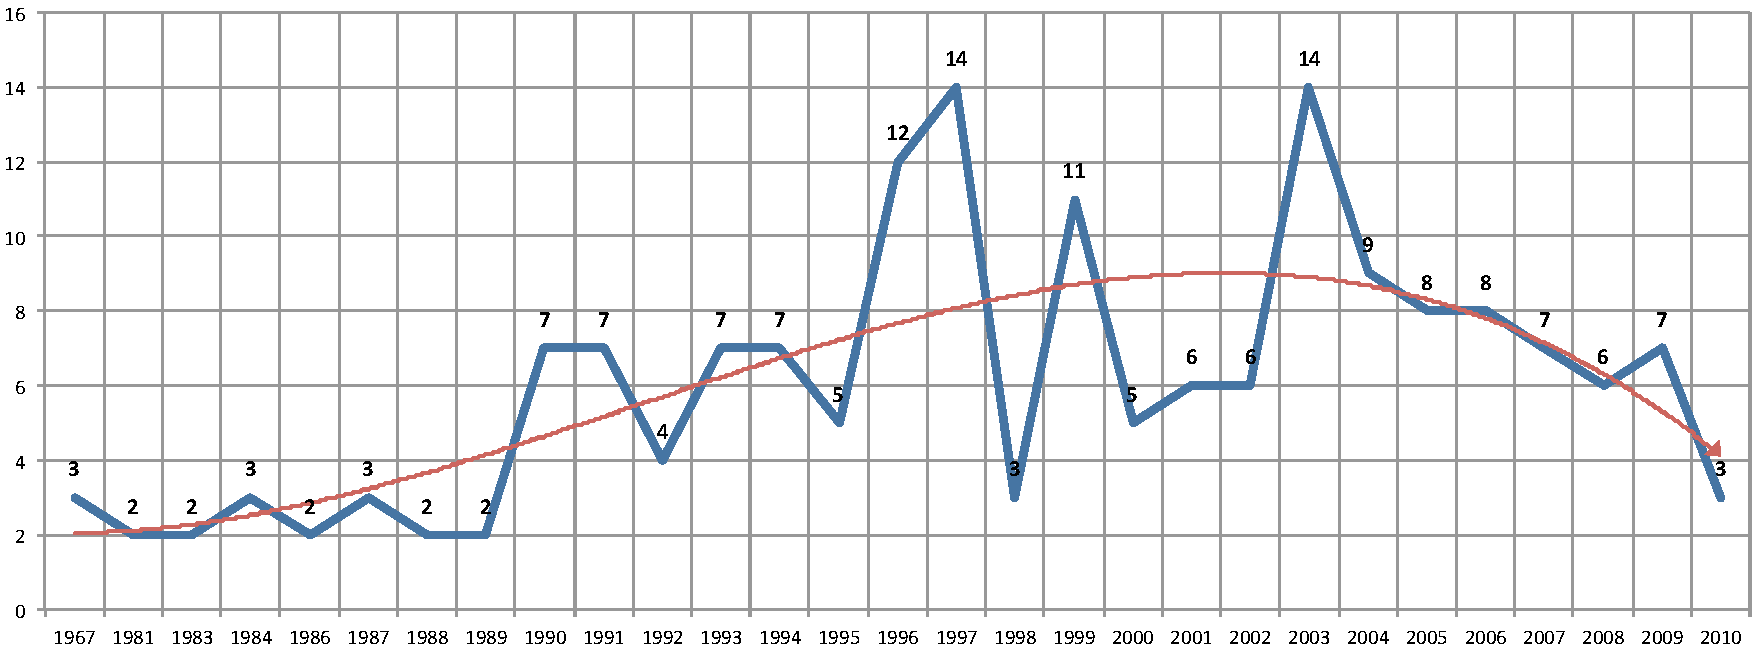
\includegraphics[scale=0.5]{ape_comandos/abntex2-modelo-img-grafico.pdf}
	\end{center}
	\caption{\label{fig_grafico}Graph produced in Excel and saved as PDF.}
	\legend{Source: \citeonline[p. 24]{araujo2012}}
\end{figure}

\section{Referencing Acronyms}

\ac{NBR} is a reference to an acronym.


%\end{apendicesenv}
% ---

% ----------------------------------------------------------
% Anexos
% ----------------------------------------------------------
% ---
% Inicia os anexos
% ---
\begin{comment}
\begin{anexosenv}
% Imprime uma página indicando o início dos anexos
\partanexos
% ---
% Incluir Anexo
% ---

%o comando lipsum[] comando serve apenas para incluir texto no documento para efeito de visualização do formato.
\lipsum[1-25]
\section{Test}
\lipsum[1-20]


\end{anexosenv}

\end{comment}


\end{document}